\documentclass[a4paper,11pt,lualatex,ja=standard]{bxjsarticle}

% 数式
\usepackage{amsmath,amsfonts}
\usepackage{bm}
% 画像
\usepackage{graphicx}
% url
\usepackage{hyperref}

% ===== cover command =====
\newcommand{\cover}[3]{
  \thispagestyle{empty}
  \vspace*{4cm}
  \begin{center}
    {\LARGE #1}\\[2cm]
    {\Large #2}\\[3cm]
    {\large 氏名：#3}\\[1cm]
    % {\large 学籍番号：s2510063}
  \end{center}
  \newpage
}
% =========================

\begin{document}

% ===== cover =====
\cover{Perceptron Train Classic 1}{SyLab}{小林智輝}
% =================

\title{レポートタイトル}
\author{氏名}
\date{\today}
\section{Perceptron Train Classic 2 Alpha}
\begin{verbatim}
Watch a perceptron learn in real time using the classic update 
rule: only misclassified points trigger updates, with no weight decay. 
In this variant you must find 5 successful learning rates (each reaching 100% accuracy) 
before the flag is revealed. Dial in a rate, trigger a run, 
and the interface animates each step. Visit the service in your browser:
\end{verbatim}

\begin{figure}[h]
  \centering
  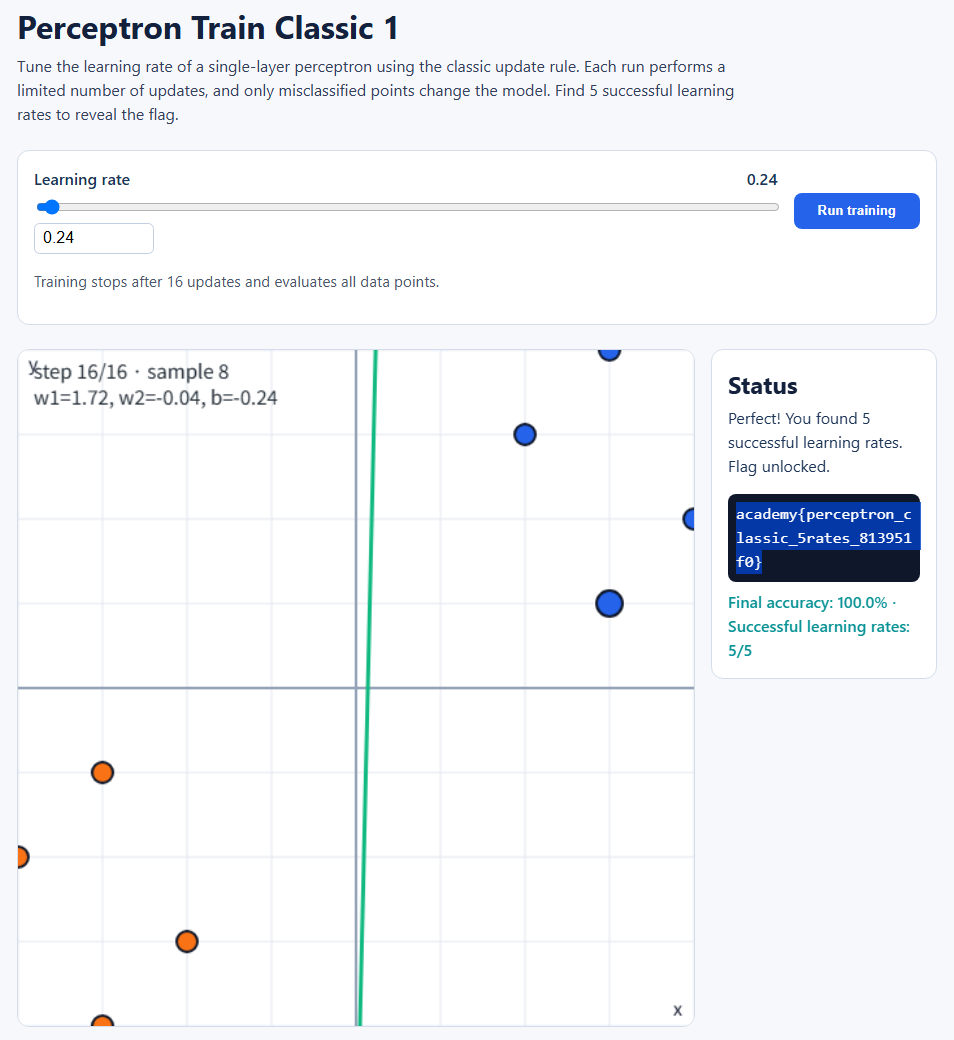
\includegraphics[width=0.7\linewidth]{05.png}
  \caption{img}
\end{figure}



\end{document}